\documentclass[tikz]{standalone}
\usepackage{tikz}
\begin{document}
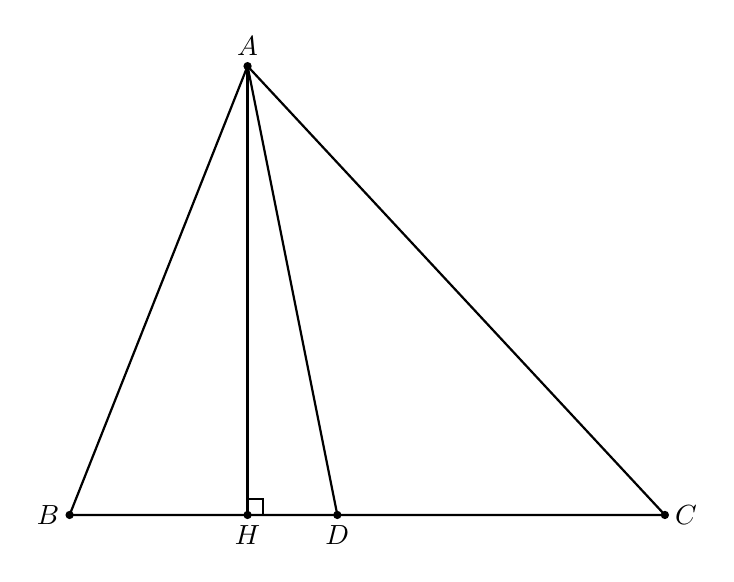
\begin{tikzpicture}[thick, scale=1]
  % 坐标 (单位 cm)
  \coordinate (B) at (0,0);
  \coordinate (C) at (7.56,0);
  \coordinate (A) at (2.26,5.7);
  \coordinate (D) at (3.4,0);
  \coordinate (H) at (2.26,0);

  % 原有线段
  \draw (A) -- (B) -- (C) -- cycle;
  \draw (A) -- (D);

  % 垂线 AH
  \draw (A) -- (H);

  % 直角标记
  \draw (H) ++(0.2,0) -- ++(0,0.2) -- ++(-0.2,0);

  % 顶点
  \fill (A) circle (1.5pt);
  \fill (B) circle (1.5pt);
  \fill (C) circle (1.5pt);
  \fill (D) circle (1.5pt);
  \fill (H) circle (1.5pt);

  % 标签
  \node[above] at (A) {$A$};
  \node[left] at (B) {$B$};
  \node[right] at (C) {$C$};
  \node[below] at (D) {$D$};
  \node[below] at (H) {$H$};
\end{tikzpicture}
\end{document}
